\documentclass{logo-cv}
% ======================== Plain version =================================== %
\newCJKfontfamily\mynamefont{Source Han Serif CN}

% ======================== University version ============================== %
\definecolor{customcolor}{RGB}{71,96,169} % 建议该颜色取自校徽
\newcommand{\aLogo}{
\includegraphics[width=0.18\textwidth]{images/logo-white.pdf}} % 页眉校徽
% 校徽可在 https://www.urongda.com/ 找到
\newcommand{\bLogo}{
\includegraphics[width=0.75\textwidth]{images/badge-blue.pdf}} % 底纹水印
\newcommand{\school}{兰州大学 | Lanzhou University} %页眉参数
\newcommand{\contact}{\textcolor{white}{\textbf{自强不息 \quad 独树一帜}}} %页脚参数


\begin{document}
\section{个人信息与教育背景}
\begin{minipage}{0.14\textwidth}
    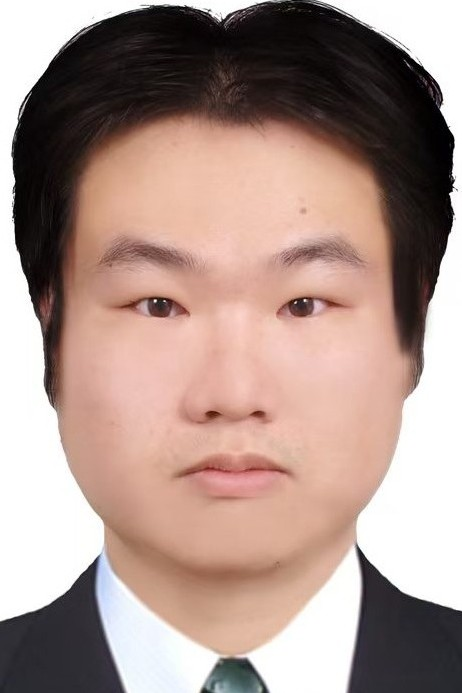
\includegraphics[height=0.7\textwidth]{images/Me_s.jpg}
\end{minipage}
\begin{minipage}{0.25\textwidth}
        \begin{tabular}{ll}
        \textbf{姓名} & {\mynamefont 许忞欢}         \\
        \textbf{电话} & 19525029181     \\
        \textbf{邮箱} & xumh2001@gmail.com \\
        \textbf{籍贯} & 江苏无锡 \\ 
        \textbf{爱好} & 业余无线电（A类）  \\ 
        \end{tabular}
\end{minipage}
\hfill
\raisebox{-0.085\textwidth}[0pt][0pt]{\textcolor{customcolor}{\rule{0.5pt}{0.17\textwidth}}}
\hfill
\begin{minipage}{0.52\textwidth}
\begin{cSubsection}{兰州大学（985工程）}{2024.9 - 至今}{信息与通信工程(前5\%)}{硕士}
\end{cSubsection}
\begin{cSubsection}{兰州大学（985工程）}{2020.9 - 2024.6}{电子信息省级基地班(\emph{前20\%, 免试攻读硕士})}{学士}
\end{cSubsection}
\end{minipage}

\section{技能}

\begin{itemize}
    \item \textbf{编程语言} \hfill 熟练使用Python, C/C++和MATLAB实现科学计算, 交互界面, 复杂逻辑等任务
    \item \textbf{硬件开发} \hfill 具备STM32开发能力；熟悉FPGA开发流程,能够使用Vivado, Vitis等工具进行FPGA设计与调试
    \item \textbf{Linux运维} \hfill 拥有Linux计算系统实际运维经验,擅长网络配置,故障排查及专业科学计算环境的搭建与检修
    \item \textbf{基础能力} \hfill 英语CET-6, 熟练使用Office办公软件以及 Origin,Visio 等作图软件
\end{itemize}

\section{科研成果}
\begin{itemize}
    \item 研究方向：非线性系统的鲁棒控制与逆强化学习
    \item 
        % \begin{itemize}
            论文《Inverse Reinforcement Q-Learning for Stochastic LQR of Nonlinear Systems》  IEEE TIE 一审大修
        % \end{itemize}
\end{itemize}

\section{项目工作}
\begin{itemize}
    \item 横向项目：通用辐射效应测试平台研制 (兰州空间技术物理研究所) \hfill 2025.10 - 至今
    \begin{itemize}
        \item \textbf{项目简介}：通过对特定信号的高速ADC采样，实现对信号的实时分析与处理,并通过FPGA对信号进行快速处理和反馈,从而实现对电子设备的辐射效应测试。
        \item \textbf{项目贡献}：负责Zynq 7000 Soc部分内容开发：PL端与PS端之间的高速数据传输、PL端的去直预处理和脉冲检测。
    \end{itemize}
    \item 横向项目：智能训练与开发平台研究 (中国航空工业集团公司雷华电子技术研究所) \hfill 2026.04 - 至今
    \begin{itemize}
        \item \textbf{项目简介}：建设一套面向雷达探测、电子干扰、侦察识别和通信等场景的智能训练与开发平台，采用“云平台—边缘计算—数字信号端”协同架构，实现高带宽、低时延、高并发信号数据处理。
        \item \textbf{项目贡献}：负责边缘计算节点和FPGA之间，基于XDMA协议的快速稳定的数据交换；同时负责基于容器技术的云平台集群主控节点和储存节点的开发，以及云端模型的部署和调度管理。
    \end{itemize}
    % \vspace{1.5cm}
    \item 保密项目：《xxxx》\hfill 2023.09 - 2025.10
    \begin{itemize}
        \item \textbf{项目简介}：xxxx
        \item \textbf{项目贡献}：作为主要软件开发者,成功完成FPGA兼GPU技术开发,系统集成与测试,并在项目中积累了丰富的实践经验。
    \end{itemize}
    \item 混沌加密图像传输 \hfill 2023.09 - 2025.10
    \begin{itemize}
        \item \textbf{项目简介}：混沌加密图像传输.
        \item \textbf{项目贡献}：为了解决FPGA平台与NVIDIA Jetson开发板直接经由PCIe接口进行数据交换的问题，针对加密算法的特殊数据要求，
        开发了一套有关彩色图像压缩，重排，整合为int32的一套转化、还原算法, 并通过C++ opencv平台对数据处理和传输进行实现。
    \end{itemize}
    \item 国家自然科学基金：《复杂环境下机器人运动控制的模仿学习技术》\hfill 2023.01 - 至今
    \begin{itemize}
        \item \textbf{项目简介}：应对在复杂情况下机器人的运动学控制,完成应用模仿学习、逆强化学习以及模型控制算法的机器人控制平台设计。
        \item \textbf{项目贡献}：设计手持控制器,结合嵌入式软件,保障便捷操作。基于QT开发上位机软件,实现友好界面与高效数据处理。针
                                对履带车底盘,优化机械设计与控制算法。探索机械臂与机械手运动学,开发精准控制策略。
                                利 用LeapMotion实现手势识别。集成多传感器技术,提升环境感知与定位。
    \end{itemize}
    \item 甘肃省重点研发计划：《机器人抗干扰高精度模型预测控制》\hfill 2025.02 - 至今 \begin{itemize}
        \item \textbf{项目简介}：研发空间灵巧手：完成非线性高精度建模, 强化学习抗干扰控制,及Transformer多任务学习
        \item \textbf{项目贡献}：为解决监督学习背景下,不可避免的复杂环境状态测量误差或对抗性噪声的问题,
        基于状态对抗马尔可夫决策过程对深度强化学习算法进行改造,通过探索最强对抗噪声,
        并在其基础上使用鲁棒策略正则化方法,建立具有强鲁棒性的强化模型预测控制系统。
    \end{itemize}
\end{itemize}


\section{本科校内工作}
\begin{itemize}
    \item 国家级大学生创新创业训练计划《基于python的<信号与系统>仿真平台设计与实现》 \hfill 2022.5 - 2023.5
    \item 计算机软件著作权《基于python的<信号与系统>连续信号仿真平台设计与实现 V1.0》 \hfill 2023.4
\end{itemize}

\section{学业荣誉}
\begin{itemize}
    \item 兰州大学优秀学生一等（2020）、二等（2021-2022）奖学金 \hfill 2020.9 - 2022.12
    \item 兰州大学优秀研究生一等（2025）、二等（2024）奖学金 \hfill 2024.9 - 2025.12
\end{itemize}

\section{自我评价}
本人具备扎实的专业基础和算法设计与实现能力,能够熟练运用C/C++,Python,MATLAB 完成建模,控制算法和UI开
发；学习能力强,善于在压力下合理安排时间,高效推进任务并解决问题；工作认真负责,注重细节,能快速
适应环境并保持持续执行力；富有团队合作精神,沟通能力良好,曾多次参与机器人开发与科研实验,积累了
丰富的实践经验。
\end{document}
